% Autor: Alfredo Sánchez Alberca (asalber@ceu.es)

\newproblem{ext-1}{gen}{*}
%ENUNCIADO
{ Below you can find the graph of the derivative $f'(x)$ of a function $f(x)$.
Determine the behaviour of $f$ (increasing, decreasing, convex, concave, extrema) from that graph.
\[
\input{img/grafica-ext-1}
\]
}
%SOLUCIÓN
{Growth: Decreasing at $(-\infty,a)$ and $(c,e)$, and increasing at $(a,c)$ and $(e,\infty)$.\\
Extrema: Minimum at $x=a$ and $x=e$, and maximum at $x=c$.\\
Concavity: Concave up at $(-\infty,b)$ and $(d,\infty)$, and concave down at $(b,d)$.
}
%RESOLUCIÓN
{
}

\newproblem{ext-2}{gen}{}
%ENUNCIADO
{Find the values of $a$, $b$ and $c$ so that the function $f(x)=x^3+bx^2+cx+d$ has an inflection point at $x=3$, its graph goes
through the point $(1,0)$, and it has a maximum at $x=1$.
}
%SOLUCIÓN
{$b=-9$, $c=15$ y $d=-7$.
}
%RESOLUCIÓN
{
}

\newproblem{ext-3}{far}{}
{A drug has to be given to patients in cylindrical pills.
The content of the drug in each pill is 0.15 ml; determine the dimensions of the cylinder so that the amount of material used to make it (the pill)
is minimal.
}
%SOLUCIÓN
{Radius $0.2879$ cm and height $0.5760$ cm.
}
%RESOLUCIÓN
{
}


\newproblem*{ext-4}{gen}{*}
%ENUNCIADO
{La variable aleatoria bidimensional $(X,Y)$ con función de densidad
\[
f(x,y) = \frac{1}{\sqrt{2\pi}\, \sigma_x\sigma_y} e^{-\frac{1}{2}\left(\frac{(x-\mu_x)^2}{\sigma_x^2}+\frac{(y-\mu_y)^2}{\sigma_y^2}\right)}
\]
se conoce como normal bidimensional con $X$ e $Y$ independientes, de parámetros $\mathbf{\mu}=(\mu_x,\mu_y)$ y $\mathbf{\sigma}=(\sigma_x,\sigma_y)$.
Calcular los puntos de inflexión de la curva formada por la intersección de la superficie de $f$ con el plano $y=x$.
}


\newproblem{ext-5}{amb}{*}
%ENUNCIADO
{A mathematical model for the amount of water in certain lake, $m(t)$, in millions of cubic meters, is given as a function of the time
$t$, measured in years lapsed since the study took place.
The formula is the following:
\[
m(t) = 10 + \frac{{\sqrt t }} {{e^t }}
\]
This formula makes sense only for positive values of the variable $t$.
\begin{enumerate}
\item How much water will there be in the lake when $t$ goes to infinity?
\item Use derivatives to find the time at which the amount of water in the lake is maximum, and compute the amount of water at such time.
\end{enumerate}
}
%SOLUCIÓN
{\begin{enumerate}
\item $\lim_{t\rightarrow \infty}m(t) = 10$.
\item $\frac{dm}{dt}=e^{-t}(\frac{1}{2}t^{-1/2}-t^{1/2})$. The moment at which the amount of water in the lake will be maximum is $t=0.5$ years and at this moment there will be $10.429$ millions of m$^3$.
\end{enumerate}
}
%RESOLUCIÓN
{
}


\newproblem{ext-6}{far}{*}
%ENUNCIADO
{Se está estudiando fabricar unas cápsulas de cuerpo cilíndrico terminadas en sus extremos por dos semiesferas. El volumen de la cápsula debe ser $0.8$ cm$^3$ y se quiere que la superficie sea mínima. ¿Cuáles deben ser las dimensiones del radio y de la longitud de la parte cilíndrica? Comentar el resultado obtenido.
\begin{quote}
    \textbf{Nota}:\\
    Volumen del cilindro $V=\pi r^2 h$\\
    Superficie lateral del cilindro $S=2\pi r h$\\
    Volumen de la esfera $V= \frac{4}{3}\pi r^3$\\
    Superficie de la esfera $S=4\pi r^2$\\
\end{quote}
}
%SOLUCIÓN
{$r = 0.5759$ y $h=0$.
}
%RESOLUCIÓN
{La capsula está formada por un cilindro de radio $r$ y altura $h$ mas una esfera (2 semiesferas) de radio $r$,
\[
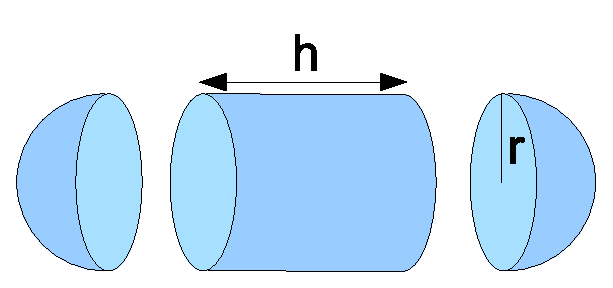
\includegraphics[scale=0.4]{img/capsula-ext-6}
\]
así que su volumen es
\[
V(r,h) = \pi r^2 h + \frac{4}{3}\pi r^3,
\]
y su superficie
\[
S(r,h) = 2\pi r h +4 \pi r^2.
\]
Como el volumen  debe ser $0.8$ cm$^3$ tenemos que
\[
V(r,h) = \pi r^2 h + \frac{4}{3}\pi r^3 = 0.8 \Leftrightarrow h = \frac{0.8-4/3\pi r^3}{\pi r^2},
\]
y sustituyendo en la fórmula de superficie tenemos
\[
S(r) = 2\pi r \frac{0.8-4/3 \pi r^3}{\pi r^2} +4 \pi r^2 = \frac{1.6-8/3\pi r^2}{r}+4\pi r^2 = \frac{1.6}{r}-\frac{8}{3}\pi r^2 +4\pi r^2 = \frac{1.6}{r^2}+\frac{4}{3}\pi r^2
\]
Como queremos que la superficie de la cápsula sea mínima, tenemos que buscar el mínimo de esta función. Para ello, calculamos primero los puntos críticos que anulan su derivada:
\[
\frac{dS}{dr} = -\frac{1.6}{r^2}+\frac{4}{3}\pi2r = 0 \Leftrightarrow \frac{1.6}{r^2} = \frac{8}{3}\pi r \Leftrightarrow \frac{8}{3}\pi r^3 = 1.6 \Leftrightarrow r^3 = \frac{1.6}{8/3 \pi} = 0.1910 \Leftrightarrow r = \sqrt[3]{0.1910} = 0.5759
\]
y por tanto la altura será
\[
h = \frac{0.8-4/3\pi r^3}{\pi r^2} = \frac{0.8-4/3\pi 0.5759^3}{\pi 0.5759^2} = 0.
\]
Esto quiere decir, que realmente no habría cilindro, y por tanto para que la supercie sea mínima la cápsula debería tener forma de esfera.

Sólo falta comprobar que el punto anterior es realmente un punto de mínimo. Para ello podemos utilizar la segunda derivada
\[
\frac{d^2S}{dr^2} = \frac{d}{dr}\left(-\frac{1.6}{r^2}+\frac{8}{3}\pi r\right) = \frac{1.6\cdot 2r}{r^4}+\frac{8}{3}\pi = \frac{3.2}{r^3}+\frac{8}{3}\pi.
\]
y sustituyendo en el punto anterior tenemos
\[
\frac{d^2S}{dr^2}(0.5759) =  \frac{3.2}{0.5759^3}+\frac{8}{3}\pi = 25.13 >0,
\]
que al tener signo positivo indica que efectivamente se trata de un mínimo.
}

\newproblem{ext-7}{gen}{*}
%ENUNCIADO
{Consider a function $f(x)$ with derivative given by
\[
f'(x) = \frac{(2-x) e^{-\frac{x^2}{2}+2x-2}}{\sqrt{2\pi}}
\]
\begin{enumerate}
\item Determine the regions on which $f$ is increasing, and those where $f$ is decreasing.
\item Find the extrema points of $f$.
\item Determine the points on which $f$ is concave up, and those on which it is concave down.
\item Find the values of $x$ corresponding to the inflection points of the graph of $f$.
\end{enumerate}
}
%SOLUCIÓN
{\begin{enumerate}
\item Increasing at $x<2$ and decreasing at $x>2$.
\item Relative maximum at $x=2$.
\item Concave down at$(-\infty,1)$ and $(3,\infty)$, and concave down at $(1,3)$.
\item Inflection points at $x=1$ and $x=3$.
\end{enumerate}
}
%RESOLUCIÓN
{
}


\newproblem{ext-8}{qui}{}
%ENUNCIADO
{The speed $v$ at which certain chemical reaction $A+B\rightarrow AB$ takes place is a function of the concentraion $x$ of the substance $AB$.
This speed it is given by the following equation:
\[
v(x) = 4(3-x)(5-x).
\]
Determine the value of $x$ that maximizes the speed of the process.
}
%SOLUCIÓN
{None.
}
%RESOLUCIÓN
{
}


\newproblem{ext-9}{amb}{}
%ENUNCIADO
{The wheat yield $C$ of a field depends on the level of nitrogen on the ground $n$, and it is given by the following relation:
\[
C(n) = \frac{n}{1+n^2},\quad n\geq 0.
\]
Find the level of nitrogen that will produce the biggest yield.
}
%SOLUCIÓN
{$n=1$.
}
%RESOLUCIÓN
{
}


\newproblem{ext-10}{amb}{}
%ENUNCIADO
{Existen organismos que se reproducen una sóla vez en su vida como por ejemplo los salmones.
En este tipo de especies, la velocidad de incremento per cápita $v$, que mide la capacidad reproductiva, depende de la edad $x$ según la ecuación
\[
v(x) = \frac{\log(p(x)h(x))}{x},
\]
donde $p(x)$ es la probabilidad de sobrevivir hasta la edad $x$ y $h(x)$ es el número de nacimientos de hembras a la edad $x$.
Calcular la edad óptima de reproducción, es decir, el valor que maximice $v$, para $p(x)=e^{-0.1x}$ y $h(x)=4x^{0.9}$.}
%SOLUCIÓN
{$x=0.58$ años.
}
%RESOLUCIÓN
{
}


\newproblem{ext-12}{amb}{}
%ENUNCIADO
{The response $S$ of an organism to a drug depends on the dose $x$ by the relation
\[
S(x) = x(C-x),
\]
where $C$ is the maximum amount of the drug that can be given to a person.
Find the dose $x$ for which the response is maximum.
}
%SOLUCIÓN
{$x=C/2$.
}
%RESOLUCIÓN
{
}
